\documentclass[conference]{IEEEtran}
\IEEEoverridecommandlockouts
% The preceding line is only needed to identify funding in the first footnote. If that is unneeded, please comment it out.
\usepackage{cite}
\usepackage{amsmath,amssymb,amsfonts}
\usepackage{algorithmic}
\usepackage{graphicx}
\usepackage{textcomp}
\usepackage{xcolor}
\def\BibTeX{{\rm B\kern-.05em{\sc i\kern-.025em b}\kern-.08em
    T\kern-.1667em\lower.7ex\hbox{E}\kern-.125emX}}
\begin{document}

\title{Experimental investigation of forced convective heat transfer in cylindrical pipe flows\\
%{\footnotesize \textsuperscript{*}Note: Sub-titles are not captured in Xplore and should not be used}
%\thanks{Identify applicable funding agency here. If none, delete this.}
}

\author{\IEEEauthorblockN{Yoshinori Hattori}
\IEEEauthorblockA{\textit{Shibaura Institute of Technology, Mechanical Engineering}\\
Tokyo, Japan \\
md18060@shibaura-it.ac.jp}}

\maketitle

% \begin{abstract}
% In recent years, forced convective heat transfer in cylindrical pipe flow has been playing an important role in many technical cooling system.
% Heat transfer coefficients are vary with flow regime.
% Much remains to be study for providing experimental data for transitional regime.
% Reliable prediction of heat transfer coefficients for transitional flow is still challenging tasks.
% In this study, I focused on forced convective heat transfer in cylindrical pipe flow for transitional regime in particular high Prandtl number.
% Moreover, the measurement of wall friction coefficients were also performed in this study.
% The engineeres is frequently interested in pressure drop which is related to determine pump or fan power equipments.
%
% \end{abstract}
%
% \begin{IEEEkeywords}
% Forced convection, Nusselt number, Wall friction, transitional, Cylindrical pipe flow
% \end{IEEEkeywords}

\section{Introduction}
In recent years, forced convective heat transfer in cylindrical pipe flow has been playing an important role in many technical cooling systems.
These coolant technology is used wide varaety of coolant applications such as electric devices, automotive, and plant factory.
Considering heat transfer issues, heat transfer coefficients are one of the most important numbers.
The Nusselt number (Nu) is a dimensionless number which represents the ratio of convective (h) and conductive heat transfer (k), as expressed in Equation \eqref{Nu_number}.
\begin{equation}
Nu=\frac{h\cdot L}{k}\label{Nu_number}
\end{equation}
For a general dimensional analysis, the Nusselt number represents function of the Reynolds number (Re) multiplied by the Prandtl number (Pr) as Equation \eqref{Nu_dimensional}.
\begin{equation}
Nu=\alpha \cdot Re^{\pi_{\beta}}\cdot Pr^{\pi_{\gamma}}\label{Nu_dimensional}
\end{equation}
Here, factors $\alpha$, $\beta$ and $\gamma$ are constant values that depend on flow regime.

In technology, flows regime and heat transfer plays an important role in considerting engineering issues.
Navie-Stokes equations describe the relation of variable flows.
However, deterministic solution of the equations are only valid for small disturbances in the initial and boundary condition.
In physically, it is hard to get initial and boundary conditions in infinite accurate.
Turbulent has a large amount of fluctuations, i.e. turbulent is completely different kind of laminar flows.
Direct Numerical Simuration (DNS) is one of the simulation way to predict flow forms.
Simuration 2 Experimental
Therefore, it is nessesary to get experimental data for correlations of heat transfer and flow condition and the Reynolds number.

Many studies have pointed out that a heat transfer coefficient varies depending on the type of flow: laminar, transition and turbulent.
Gnienlinski\cite{Gnienlinski2010} showed a calculation method for the laminar heat transfer coefficient under two kinds of boundary conditions: constant wall temperature (I) and constant heat flux (I\hspace{-.1em}I).
Petukhvov and Kirillov\cite{Petukhov1958} showed calculation method for turbulent flows.
Not so many data is available for experimental data of laminar-to-turbulent transitional region.
Bertsche et al.\cite{Bertsche2016} focused on reliable prediction of the heat transfer coefficient for transitional flows.
In their study, they showed experimental the heat transfer coefficients for the Reynolds number, $500 < Re < 23000$, and the Prandtl number, $7 < Pr < 41$.

More studies should be conducted to obtain experimental data for high the Prandtl number and transitional flows.
In this study, the author focused on forced convective heat transfer in flow of water and glycole in a cylindrical pipe.
A 50/50vol\% mixture of water and glycole, which is a typical liquid coolant in automotive applications, was used as an operating fluid.
The experiment was carried out by considering a board range of Reynolds numbers, spanning from a laminar to fully turbulent flow.
Moreover, the measurements of the wall friction coefficients was also performed in this study.
The experimental data were compared with other sources as well as computational results obtained from already existing numerical simulations (CFD) by Christphan \cite{Christphan2018}.


% \section{The phenomena}
% %Temperature variations for constantHeat flux
% \begin{figure}[htbp]
%  \centering
%  %\vspace{-3zh}
%  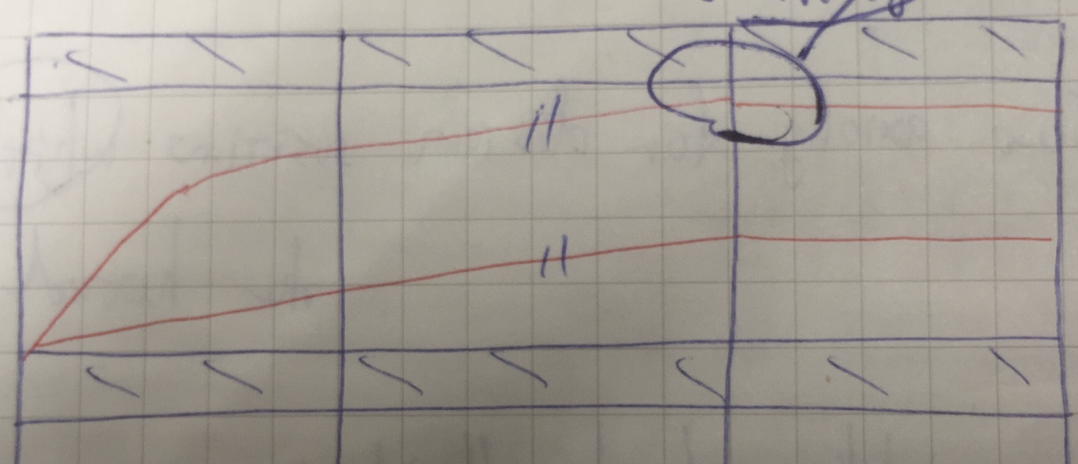
\includegraphics[width=0.47\textwidth,natwidth=610,natheight=642]{fig/temperature_variations_constant_heat_flux.png}
%  \caption{Temperature variations for constantHeat flux}
%  \label{temperature_variations_constant_heat_flux}
% \end{figure}
%
% %Heat transfer coefficient depend on x value
% Figure\label{heat_transfer_coefficient_depend_on_x_value} shows the local heat transfer coeeficient
% \begin{figure}[htbp]
%  \centering
%  %\vspace{-3zh}
%  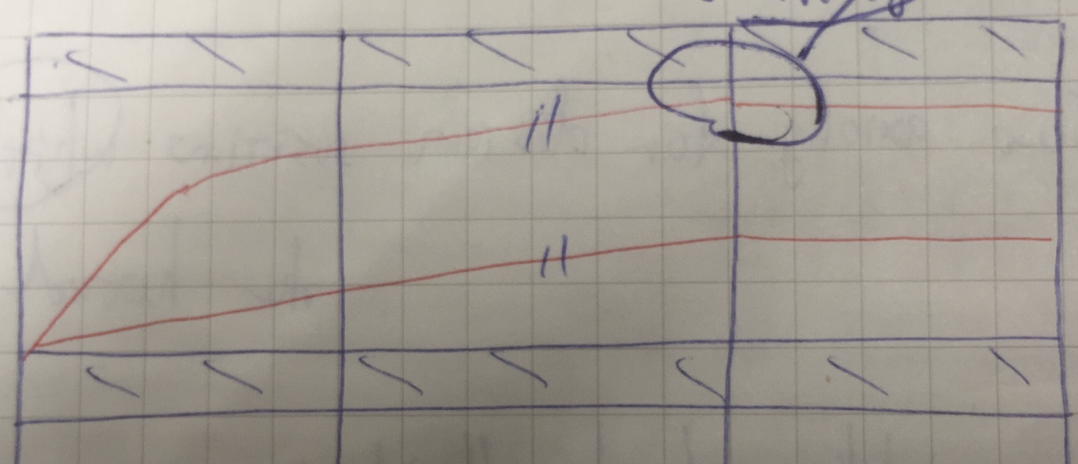
\includegraphics[width=0.47\textwidth,natwidth=610,natheight=642]{fig/temperature_variations_constant_heat_flux.png}
%  \caption{Heat transfer coefficient depend on x value}
%  \label{heat_transfer_coefficient_depend_on_x_value}
% \end{figure}
% There are two surface conditions arise in many engineering applications.
% One is constant surface heat flux and the other is constant surface temperature.
% In the fully developed flow of the tube, fluid constant porperties, the local heat coefficient is constant independent of x.


\section{Emperical correlations}
\subsection{The friction coefficients}
The skin friction coefficients for laminar flow is descrived following equation.
\begin{equation}
    C_{f,lam}=\frac{16}{Re_{b}}
    \label{cf_laminar}
\end{equation}
Konakov\cite{Konakov1954} showed the skin friction coefficients for turbulent flow.
\begin{equation}
    C_{f,turb}=0.25(1.8log(Re_{b})-1.5)^{-2}
    \label{cf_turbulent}
\end{equation}


\subsection{The heat transfer coefficients}
Gunienski\cite{Gnienlinski2010} showed correlations for each flow conditions: laminar, transitional and turbulent, respectively.
Gunienski\cite{Gnienlinski2010} showed calculation method for laminar flow.
\begin{equation}
    Nu_{lam}=(3.66^{3}+0.7^{3}+(1.615(Re_{b}Pr_{b}\frac{d_{i}}{L})^{1/3})^{3})^{1/3}
    \label{Nu_laminar}
\end{equation}
%The range 0.1<<Pr_{b}<<1000, 10^{4}<<Re_{b}<<10^{6}.
He showed calculation method for turbulent flow.
\begin{equation}
    Nu_{turb}=\frac{\frac{C_{f,turb}}{2Re\cdot Pr_{b}}}{1+12.7 \sqrt{\frac{C_{f,turb}}{2}}(Pr_{b}^{2/3}-1)}\cdot (\frac{Pr_{b}}{Pr_{w}})^{0.11}
    \label{Nu_turbulent}
%Nu_{turb}=\frac{\frac{C_{f}}{2\cdot Re\cdot Pr_{b}}{(1+12.7\frac{C_{f}}{2}}\cdot (Pr^{\frac{2}{3}}-1)}\cdot(1+(\frac{d_{h}}{l})^{\frac{2}{3}})\label{Nu_turblent}
\end{equation}
The range is
\begin{equation}
    0.1<<Pr_{b}<<1000, 10^{4}<<Re_{b}<<10^{6}
\end{equation}
He presented transitional flow as a liner interpolation between turbulent and laminar flow.
\begin{equation}
    Nu_{m}=(1-r)Nu_{m,lam}+rNu_{m,turb}
    \label{Nu_transitional}
\end{equation}
\begin{equation}
    r=\frac{Re_{b}-2300}{10^{4}-2300}
\end{equation}


\section{Experimental setup}
%Experimental Setup
Figure. \ref{experimental_loop} shows a diagram of the experimental loop.
The experimental basically loop consists of a heat exchanger, a pump, a Coriolis mass flow rate, a welder, a reservoir, and a test section.
The heat exchanger keeps a thermal stationary condition in the flow pipe.
The Coriolis mass flow rate is controlled by the pump and a bypass valve C, which is located in parallel to the pump.
The pipe is thermally insulated by using glass wool.\\

\begin{figure}[htbp]
\centering
\vspace{-4zh}
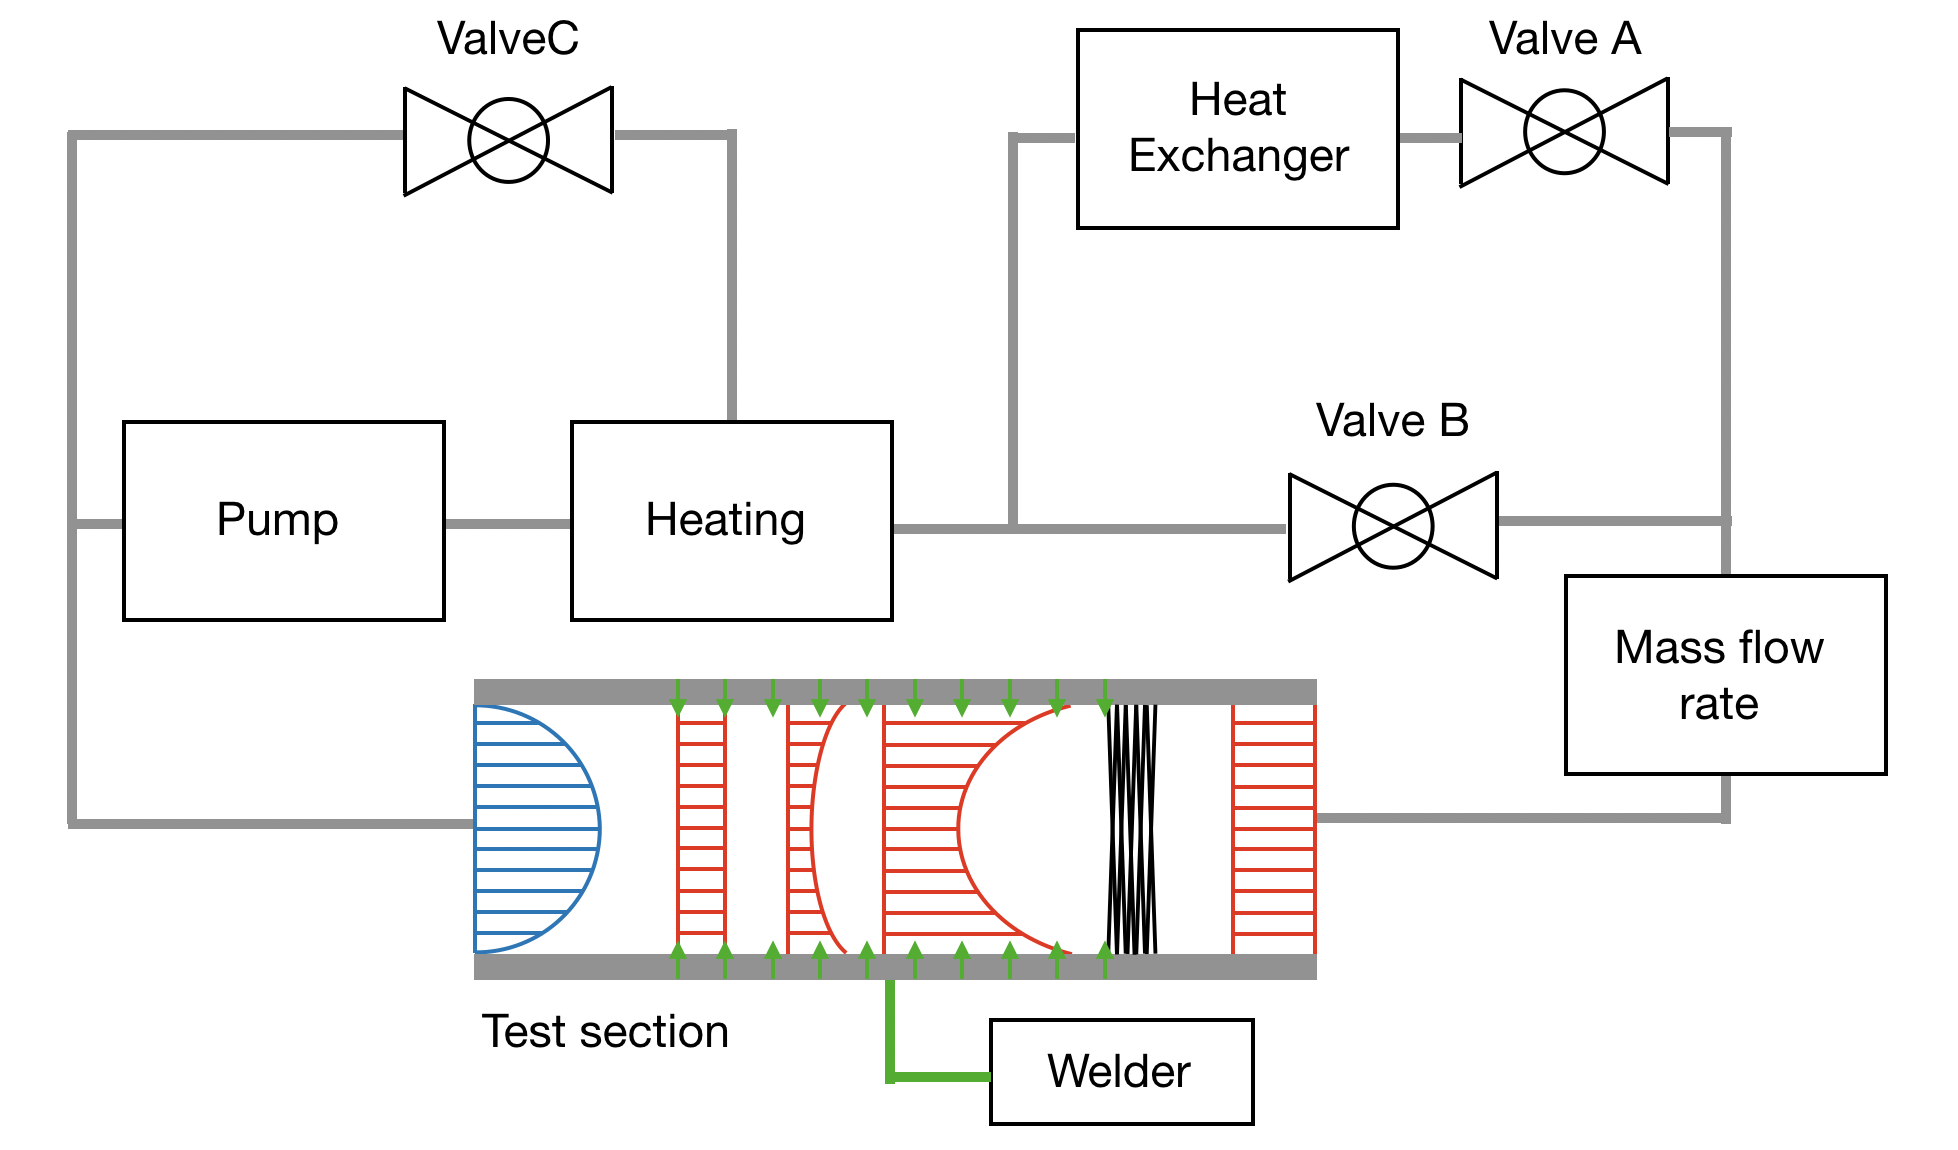
\includegraphics[width=0.47\textwidth,natwidth=920,natheight=700]{fig/experimental_loop.png}
\caption{Process flow diagram of the test facilities including test section.}
\label{experimental_loop}
\end{figure}

Figure. \ref{thermal_boundary_layer_development} shows the velocity and thermal boundary layer of developments vary with the horizontal axis in the test section.
%thermal boundary layer of WHAT???
The velocity and thermal profiles are shown in blue and red color, respectively.
The test section is made of stainless steel (1.4301) with an inner diameter di=12mm and outer diameter do= 15mm.
Highly accurate resistance thermall probes (PT-100) are used to find out the inlet and outlet bulk temperatures (Tib , Tob) and wall temperature (Tw).
Moreover, thermocouples (Type-K) are used to measure temperature gradients in the flow direction.

The test section consists of entrance, heated and thermal equalized parts.
\begin{enumerate}
  \item Entrance part\\
  The first part of the test section is a 1.2 [m] length entrance part, which is sufficiently long to ensure producing dynamically developed flow condition at the exist.
  The bulk temperature (Tb0) at this section was measured by PT-100.
  \item Heated part\\
  The second part of the test section is a 2 [m] length heated part, which is sufficiently long to ensure producing thermal fully developed flow condition at the exist.
  The tube wall were heated electrically by the welder which provides high current and low voltages to keep the uniform heat flux condition in a inner pipe flow.
  Convective heat transfer is independent of the horizontal axis in fully developed flow and constant heat flux condition.
  The wall temperature (Tw) at the end of this section were measured by PT-100.
  \item Thermal equalized part\\
  The third part of the test section is the thermall equalized part, which includes a Static mixture.
  The static mixture forms turbulent and vortex.
  Then, the thermal gradients of fluids become averaged, and bull temperature (Tb1) is measured.
\end{enumerate}

\begin{figure}[htbp]
  \centering
  %\vspace{-3zh}
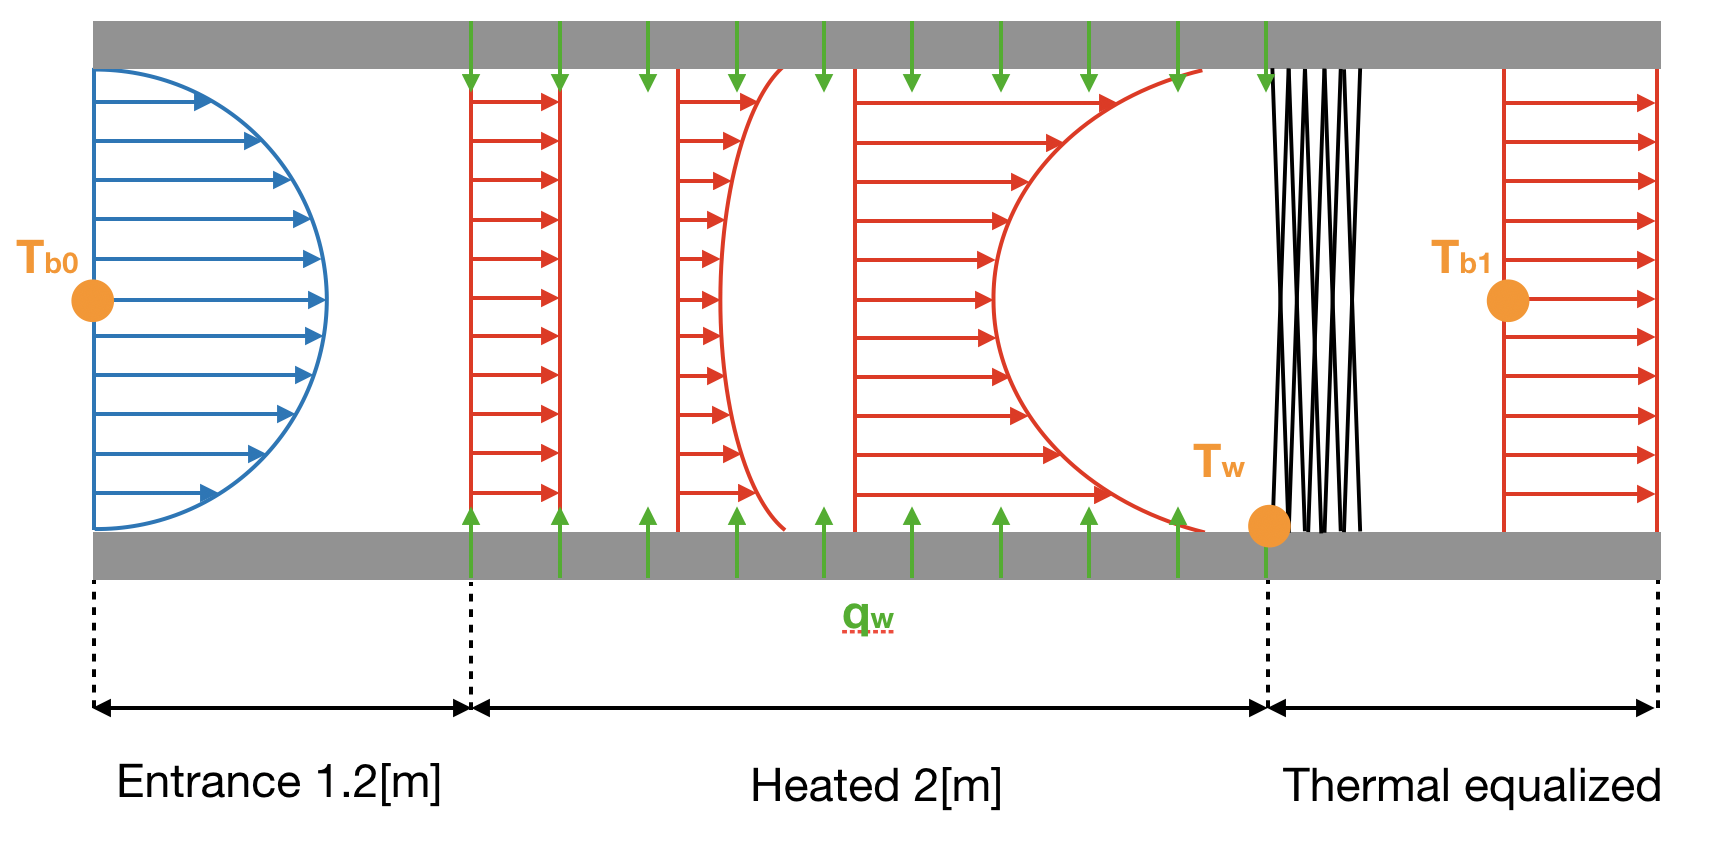
\includegraphics[width=0.47\textwidth,natwidth=850,natheight=450]{fig/thermal_boundary_layer_development.png}
  \caption{Velocity (blue) and thermal (red) boundary layer development vary with horizontal axis in a test section.}
  \label{thermal_boundary_layer_development}
\end{figure}


\subsection{Length-to-diameter ratio}
%Ref. Experiments in Pipe Flows at Transitional and Very High Reynolds Numbers p25-
The length-to-diameter ratio is an important parameter to achieve the fully developed turbulent condition in the test section.
Test section has an inner diameter of $d_{i}=12mm$, and the length of $L=2m$ which length-to-diameter ratio is $L/d_{i}=167$.
Patel et.al.\cite{Patel1969} showed suitable the length-to-diameter ratio for fully developed turbulent flows.
According to their study, they found that the minimum developing length of $L/d_{i}=70d_{i}$.
Therefore, the length-to-diameter ratio of the test section in this experimental is long enough to ensure the fully developed turbulent flow state.

%\subsection{Conduction equation}
%TPT100 sensors are attached

\subsection{Wall roughness}
%Wall properties
To clarify the wall surface as a smooth pipe, wall roughness was considered.
Moody diagram defined the basis of friction chart, and that can be used in practice.
Nikuradse made a throughout studies of turbulent flows in pipes with a rough surface.
Reynold number can be interpreted as the ratio between the rough height $h$ and thickness of the viscous sublayer $\nu/u_{*}$, as the following equation.
\begin{equation}
    Re=\frac{hu_{*}}{\nu}
\end{equation}
Here, $u_{*}$ represents wall friction velocity and descrived following equation.
\begin{equation}
    u_{*}=\sqrt{\frac{\tau_{wall}}{\rho_{0}}}
\end{equation}
Wall roughness of a characteristic height is descrived following equation.
\begin{equation}
    h = 4k_{rms}
\end{equation}
In this experiment, the surface roughness of interior surfaces in stainless steel (1.4301) is approximately $k_{rms} = 5\mu m$.\\
Table\ref{wall_roughness} shows roughness consideration in this experiment.
%at maximim Re number
\begin{table}[h]
    \caption{Oders of each terms in Equation}
    \label{wall_roughness}
    \centering
    \begin{tabular}{ccccc}
        \hline
        surface roughness & roughness height & viscous sublayer & Re \\
        \hline
        5$\mu m$ & 20$\mu m$ & 0.4$\mu m$ & 0.48
    \end{tabular}
\end{table}
It is shown that the Reynolds number in this experiment is less than 1.
Thus, the interior wall surface in the experimental setup is considered to be a smooth surface.

\subsection{Velocity profiles}
Turbulent velocity profiles for the smooth wall as following equation.
\begin{equation}
    \overline{u} = u_{*} \left[\frac{1}{k}ln\left(\frac{y}{h}\right)+B^{\prime}\right]
\end{equation}
$B^{\prime}$ is a function of the Reynolds number and calcurated as following equation.
\begin{equation}
    B^{\prime} = 2.5 ln\left(\frac{hu_{*}}{\nu}\right)+5
    %for :\frac{hu_{*}}{\nu}<<1 (i.e. a smooth wall)
\end{equation}

Figure\ref{mean_velocity_profile} shows mean velocity profile when Re = 2300 and Pr = 50.
\begin{figure}[htbp]
  \centering
  \vspace{5zh}
  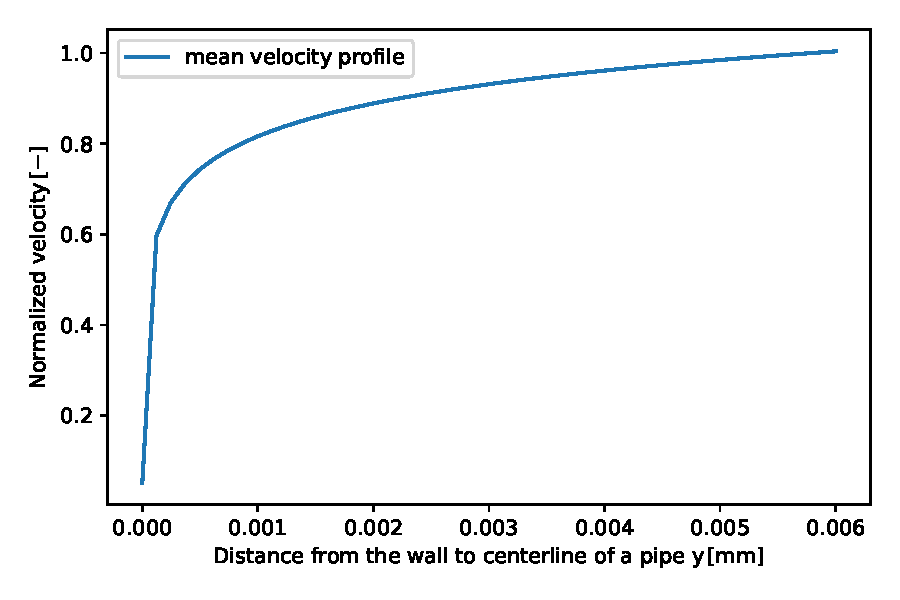
\includegraphics[width=0.47\textwidth, natwidth=400,natheight=200]{fig/velocity_profile.pdf}
  \vspace{-1zh}
  \caption{mean velocity profile when Re=2300 and Pr=50.}
  \label{mean_velocity_profile}
\end{figure}

\section{Effective data procedure}


\section{Calucuration Flow}
Since all materials can be expressed by temperature-dependent functions.
At first, the author measured the material properties of density $\rho$,  heat conductivity $k$, specific heat transfer $Cp$, kinetic viscosity $\nu$, dynamic viscosity $\mu$, Prandtl number $Pr$ that depend on temperature.
Next, he measured temperature differences, pressure differences and mass flow rates of the test section.
Finaly, Nusselt, Prandtl, Reynolds numbers and friction coefficients were calcurated by post-proccesing with LabView and MATLAB.
Figure\ref{post_processing} shows ----
\begin{figure}[htbp]
  \centering
  \vspace{-6zh}
  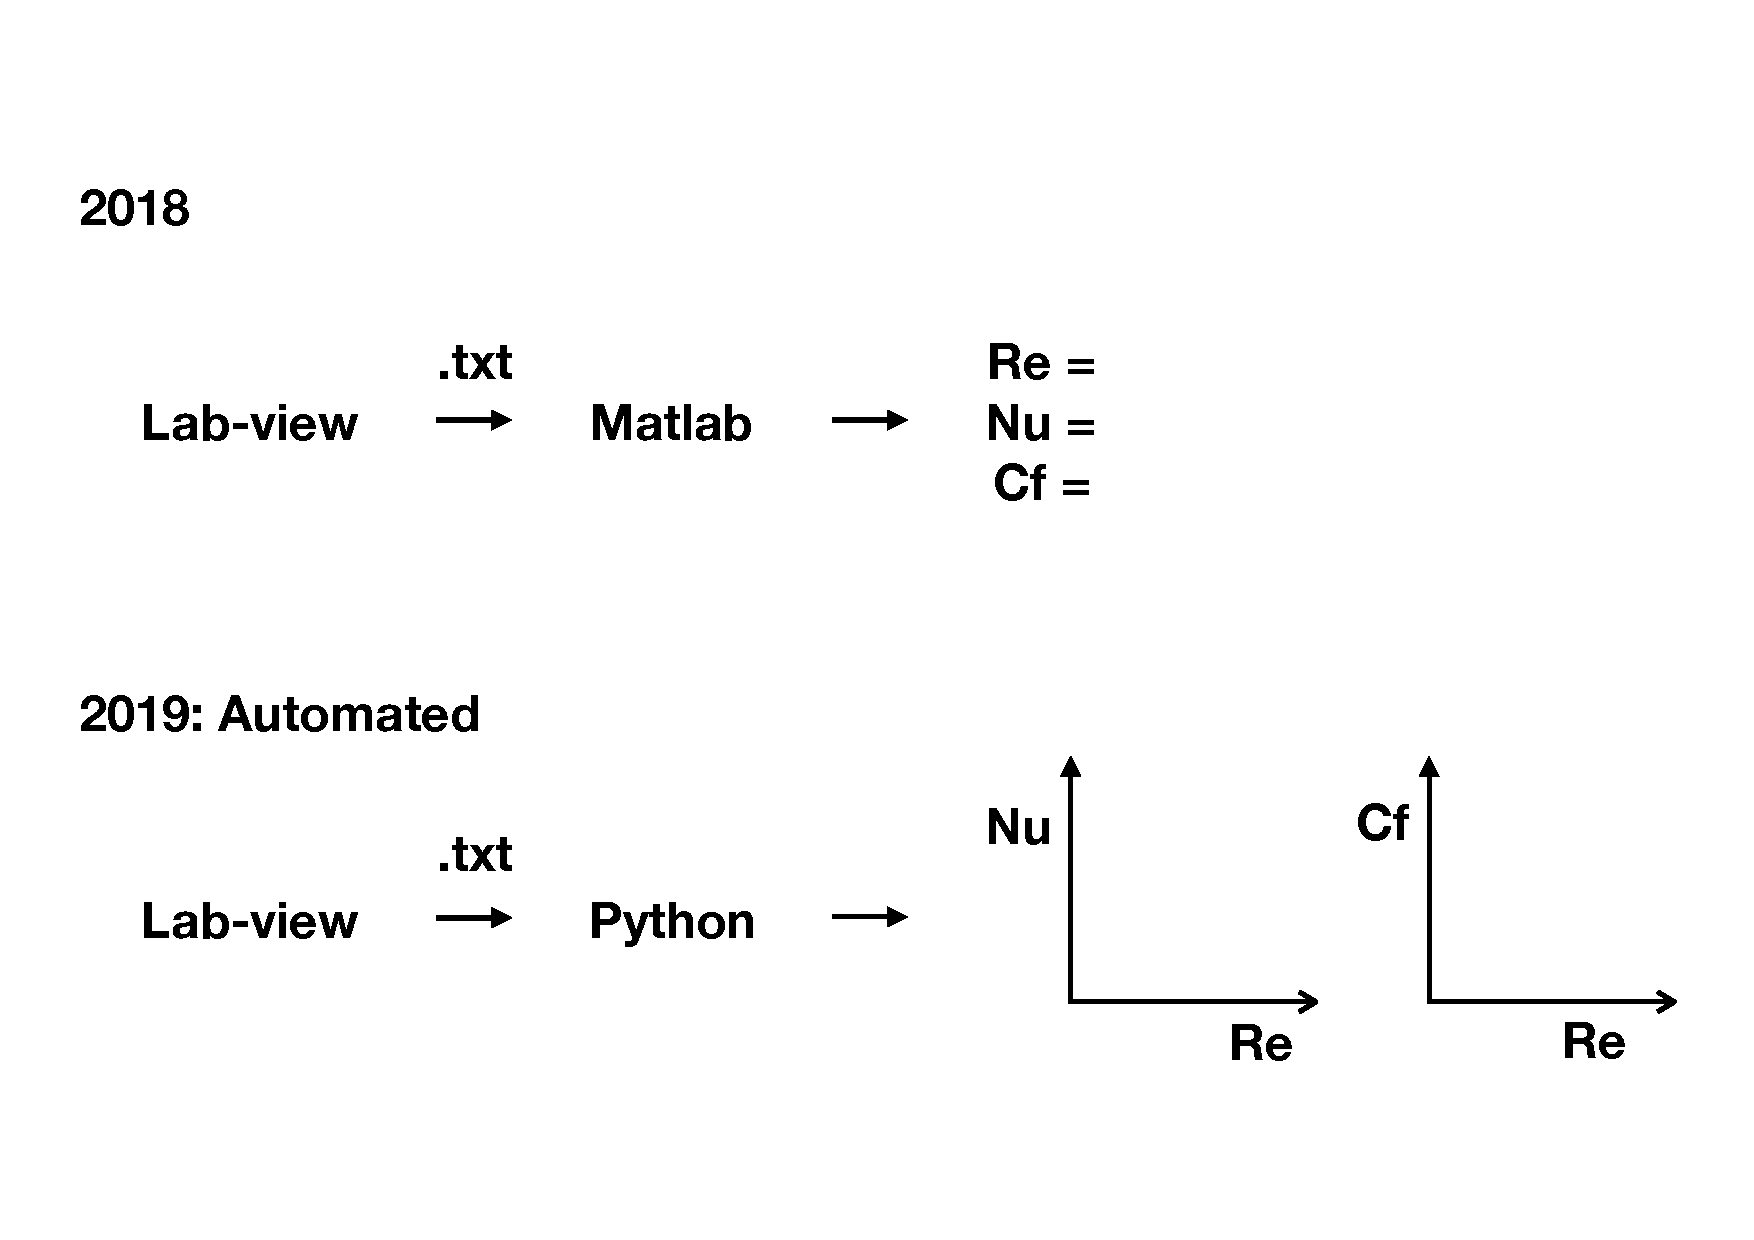
\includegraphics[width=0.56\textwidth, natwidth=920,natheight=720]{fig/post_processing.pdf}
  \vspace{-3zh}
  \caption{Developed improvement post processing compared with 2018}
  \label{post_processing}
\end{figure}

\newpage
\newpage
\section{Results and Discussions}
Data obtained in previous study\cite{Christphan2018} using the same experimental facilities indicated that heat transfer and friction coefficients for Shell Heat Transfer Oil.
Bertsche et al.\cite{Bertsche2016} showed heat transfer coefficiets for $500 < Re < 23000$ and $7 < Pr < 41$ with $80.8\%$ data for water-glycole mixture with a mass friction of water of $x_{m} = 0.477$.
According to their study, experimental data were within $\pm15\%$ to the emperical equations (\ref{Nu_laminar})(\ref{Nu_turbulent})(\ref{Nu_transitional}).
The aim of this research is to investigate heat transfer and friction coefficients using  water-glycole $50\%/50\%$ mixture as an oparatiog liquid.
In order to investigate Prandtl number throughly, first the experimental results for Pr=50 is compared with data obtained in previous studies \cite{Christphan2018} using Shell Heat Transfer Oil for Prandtl numbers Pr=50.
Therefore, the validity of evaluation process for the experiment are checked.\\

%\subsection{Heat transfer coefficients for $Pr=50$}
Figure. \ref{renu_pr50} shows dimensionless heat transfer coefficients for $Pr=50$ compared to emperical correlations equations (\ref{Nu_laminar})(\ref{Nu_turbulent})(\ref{Nu_transitional}) and previous studies.
\begin{figure}[htbp]
  \centering
  \vspace{5zh}
  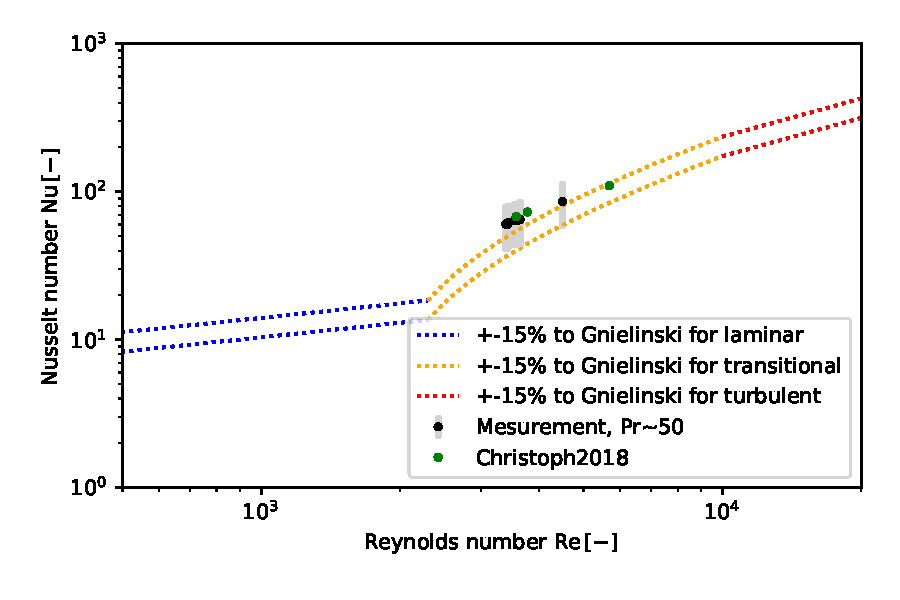
\includegraphics[width=0.47\textwidth,natwidth=400,natheight=200]{fig/renu_pr50.pdf}
  \vspace{-1.5zh}
  \caption{Dimensionless heat transfer coefficients compared to literature data and previous studies for Pr = 50. The red, yellow and blue lines are Gnielinski correlations for laminar, transitional and turbulent, respectively.}
  \label{renu_pr50}
\end{figure}\\

%\subsection{Friction coefficients for $Pr=50$}
Figure. \ref{recf_pr50} shows friction coefficients compared to emperical correlations equations(\ref{cf_laminar})(\ref{cf_turbulent}) and previous studies.
\begin{figure}[htbp]
  \centering
  \vspace{5zh}
  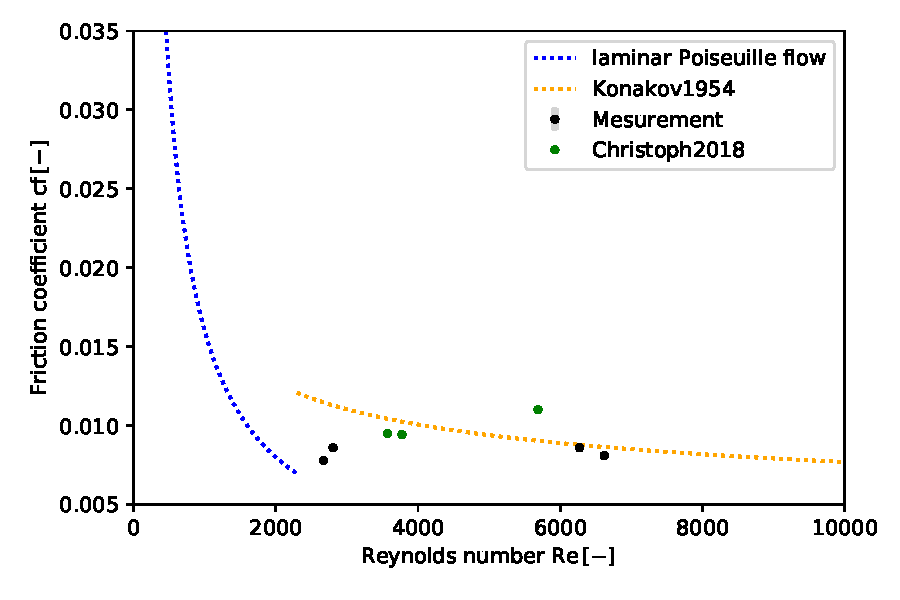
\includegraphics[width=0.47\textwidth,natwidth=400,natheight=200]{fig/recf_pr50.pdf}
  \caption{Friction coefficients compared to literature data for Pr = 50. The red and blue lines are emperical correlations for laminar and turbulent flows, respectively.}
  \label{recf_pr50}
\end{figure}
As cen bee seen, it is obvious that the experimental results on friction coefficient for $2200 < Re < 7000$ are very well fitted by the citted correlations, which is consistent with results obtained in previous studies.
However, the data for heat transfer were not consistent with these result for transitional flow regime.
Although heat transfer for higher-transitional flow regime were in line with those of Gnielinski\cite{Gnienlinski2010} correlations, a striling difference was noted for lower-transitional flow regime.\\
%A problem of Prandtl isnt constant.
Since all material properties can be expressed by temperature-dependent functions, it is difficult to keep a high Prandtl number and a transitional Reynolds number.
For example, as enhance cooling, statics viscosity increase.
As a result, the Prandtl number increase and the Reynolds number decrease.
Those numbers are related.
In correlations, the Prandtl number was assumed to be constant value.
However, the experimental Prandtl number was not constant because the fluid properties vary with temperature.
In this study, the author tried to keep the Prandtl number constant but it was not achieved.
Thus, he plot the heat transfer and the Reynolds number for the Prandtl number as devide some cases.


%\subsection{Uncertainty analysis}
A quantitative analysis to determine mesurement uncertainties was applied,
based on estimating the maximum possible error in the parameters evaluated from mesurement data.
The uncertainty of measurement was analyzed by using ``Guide to the Expression of Uncertainty in Measurement``(GUM).
Nusselt number is calcuretad from Equation (\ref{Nu_calcuration}).
\begin{equation}
    Nu=\frac{\dot{m} c_{p}(T_{1}-T_{0})}{\lambda (T_{w}-T_{1}) d\pi L}\label{Nu_calcuration}
\end{equation}
The uncertainty in Nusselt number is calcurated from Equation (\ref{Nu_uncertainty1}).
\begin{equation}
    Nu=\sqrt{\sum \left(\frac{\partial Nu}{\partial X_{i}} \Delta X_{i}\right)^{2}}\label{Nu_uncertainty1}
\end{equation}
Each parameter, X effects each parameters of Equation (\ref{Nu_calcuration}).
Then, the mesurement uncertainty in Nusselt number leads to Equation (\ref{Nu_uncertainty2}).
\begin{equation}
    \begin{split}
        &\frac{\Delta Nu}{Nu} =\sqrt{\left(\frac{\Delta \dot{m}}{\dot{m}}\right)^{2}+\left(\frac{\Delta c_{p}}{c_{p}}\right)^{2}+\left(\frac{\Delta \lambda}{\lambda}\right)^{2}}\\
        &\quad +\left(\frac{\Delta T}{T_{0}-T_{1}}\right)^{2}+\left(\frac{\Delta T(T_{0}-T_{w})}{(T_{0}-T_{1})(T_{1}-T_{w})}\right)^{2}+\left(\frac{\Delta T}{T_{1}-T_{w}}\right)^{2}\\
        \label{Nu_uncertainty2}
    \end{split}
\end{equation}

The mesurement uncertainty in friction coefficients leads to Equation (\ref{cf_uncertainty})
\begin{equation}
    \frac{\Delta C_{f}}{C_{f}} = \sqrt{\left(\frac{\Delta P}{P}\right)^{2}+\left(\frac{\Delta \rho}{\rho}\right)^{2}+2\left(\frac{\Delta \dot{m}}{\dot{m}}\right)^{2}}
    \label{cf_uncertainty}
\end{equation}
Based on this approach, the average uncertainty of the mesurement for this study shows --
Nevertheless, these results suggest that


\subsection{Purpose of the solution to deduce mesurement uncertainty for Nu}
Table (\ref{order}) shows the orders of each terms in Equation \ref{Nu_uncertainty2}.
From this comprehensive result, temperature term is several orders of magnitude larger than others.
Therefore, temperature mesurement is strongly inflected to mesurement uncertainty.
%for the high-order terms are considerd to be less important than those of low order terms.
According to this analisis, careful selections of temperature sensors are needed.
\begin{table}[h]
 \caption{Oders of each terms in Equation \ref{Nu_uncertainty2}.}
 \label{order}
 \centering
 \begin{tabular}{ccccc}
\hline
      & Mass flow & Specific heat capacity & lambda & Temperature \\ \hline
Order & O (-8)    & O (-8)                 & O(-8)  & O(-4)
 \end{tabular}
\end{table}

\section{Future plan}
An operating fluid was changed from Shell Heat Transfer to Water-glycol.
And new accurate thermocouples were repalaced.
The author describes future plans below.
\begin{enumerate}
  \item Modify Labview program for the new thermocouples
  \item Take material properties for water-glycole
  \item Check validity of the result with Bertsche et al.\cite{Bertsche2016}.
  They showed heat transfer coefficiets for $500 < Re < 23000$ and $7 < Pr < 41$ for water glycol mixture
  \item Focus on transitional and high Prandtl number
  \item Compare with already existing numerical simurations (CFD) and empirical correlations
  \item Documentation
\end{enumerate}

\newpage
\section{Appendix}
The experiment was carried out already existing fasilities by Christphan2018 \cite{Christphan2018}.
Experimental procedure is as follows.
\begin{enumerate}
  \item Switch on (Ein) Main switch (S0)
  \item Start up a computer
  \begin{enumerate}
      \item Select ``Rohro.lvproj''
      \item Select Lab VIEW and click ``Starten''
      \item Click ``Nein''
      \item Select ``Rohrpufsp.vi''
  \end{enumerate}
  \item Prepare water supply for cooling experimental facilities.
  \begin{enumerate}
      \item Open the tap water and save cool water in big tank.
      \item Cehck the temperature is approximately 15$^\circ$C.
      \item Cehck the valves are in following state.
      Valve A is closed, B is opened, and C is closed.
      \item Turn on pump swith to supply cooling water
  \end{enumerate}
  \item Check the value of mass flow rate on PC display and wait until the value is approximately 0.
  \item Click $T_{s}$ allec and $T_{s}$ gleci to carry out Temperature calibration
  \item Switch on heater (S1: Heizstab)
  \item Click ``Aushmine'' to start the experiment
  \item Set ``Welder stom'' under 300A
  \item Switch on the pump (S4: Pump)
  \item Switch on the welder
  \item Adjest suitable experimental parameters for Re and Pr.
  \begin{enumerate}
      \item Decrease Re and increase Pr\\
      %Open valve A and close valve B little by little.
      %Enhance cooling, statics viscosity increase.
      %Thus, Pr increase.
      \item Decrease Re and decrease Pr\\
      \item Decrease Re and keeps Pr constant\\

  \end{enumerate}
  \item Wait until the condition reaches steady
  \item Click ``Schreiben'' to save the data
  \item Switch of the Welder
  \item Open the valves (flow max) and cool down the facilities
  \item Wait until the facilities cool down enough
  \item Turn off pump swith to stop supplying cooling water
  \item Switch off the pump (S4: Pump)
  \item Close the tap water
  \item Click ``close'' for LabView application
  \item Shut down PC and click ``Klick sie heir unclear----'', not to download any current version
\end{enumerate}

\begin{thebibliography}{00}
%\bibitem{Frank} Frank P. Incropera, David P. DeWitt, ``Fundamentals of Heat and Mass Transfer,'' 4th edition., WILEY, 1996.
\bibitem{Patel1969}Patel and Head
\bibitem{Konakov1954}Konakov
\bibitem{Gnienlinski2010} V. Gnienlinski, ``Heat Transfer in Laminar Flow,'' VDI Heat Atlas, second ed., Springer Verlag, 2010 (Chapter Ga 1-7), Section 3.
%\bibitem{Petukhov1958} B.S. Petukhov, V.V. kirillov, Teploenergetika 4 (1958) 91-98.
\bibitem{Bertsche2016} Dirk Bertsche, Paul Knipper, Thomas Wetzel, ``Experimental investigation on heat transfer in laminar, transitional and turbulent circular pipe flow,'' International Journal of Heat Transfer, 95 (2016) 1008-1018.
\bibitem{Christphan2018} Christphan, ``Title of paper if known,'' unpublished, 2018.
\bibitem{Emir2018}Emir Öngüner, 'Experiments in Pipe Flows at Transitional and Very High Reynolds Numbers', Cuvillier Verlag, 2018.
\bibitem{Petukhov1958}Petukhov


%bibitem{Konakov1954} Konakov, ``Eine neue Formel fr den Reibungskoezienten glatter Rohre,'' Bericht der Akademie der Wissenschaften der UDSSR 51.7, 503-506.

% \bibitem{b5} R. Nicole, ``Title of paper with only first word capitalized,'' J. Name Stand. Abbrev., in press.
% \bibitem{b6} Y. Yorozu, M. Hirano, K. Oka, and Y. Tagawa, ``Electron spectroscopy studies on magneto-optical media and plastic substrate interface,'' IEEE Transl. J. Magn. Japan, vol. 2, pp. 740--741, August 1987 [Digests 9th Annual Conf. Magnetics Japan, p. 301, 1982].
% \bibitem{b7} M. Young, The Technical Writer's Handbook. Mill Valley, CA: University Science, 1989.

%\bibliography{junsrt}
%\bibliography{project_forced_convective@Graz.bib}

\end{thebibliography}
%\vspace{12pt}
%\color{red}
%IEEE conference templates contain guidance text for composing and formatting conference papers. Please ensure that all template text is removed from your conference paper prior to submission to the conference. Failure to remove the template text from your paper may result in your paper not being published.

\end{document}
